\chapter{Conception}

La phase de conception est la phase la plus crucial du processus de développement d’une application. En effet, cette phase vise à transformer un concept abstrait en un produit réel. Un projet bien conçu est facile à implémenter et à maintenir. Ainsi, le choix de la conception à adopter est très important afin de mettre au point un système convivial. Ainsi ce chapitre sera consacré à la présentation des différentes étapes de la conception de notre application, et afin de présenter au mieux cette partie nous allons donner une vue globale décrivant le schéma de la solution projetée, la procédure à suivre, l’architecture générale, et la décomposition logique de l’application. Dans une deuxième partie de ce chapitre nous allons utiliser le langage semi-formel UML\cite{cite1} pour illustrer le diagramme de classe et le diagramme entité-relation de la base de données.
\section{Conception générale}
Il est primordiale à la conception de tout système informatique de choisir l’architecture qui lui sera adéquat assurant son bon fonctionnement.

\subsection{Schéma de la solution projetée}
Puisque le système s’exécute sur une architecture réseau bien déterminée et conçu auparavant, on a recours donc à prendre en compte lors de la phase de conception architecture, c’est pourquoi nous proposons une solution qui envoie les requêtes d’apurement sur le réseau existant en mode distribution. L’acheminement des requêtes est présenté par la figure 5.1. 
\begin{figure}[!h]
\begin{center}
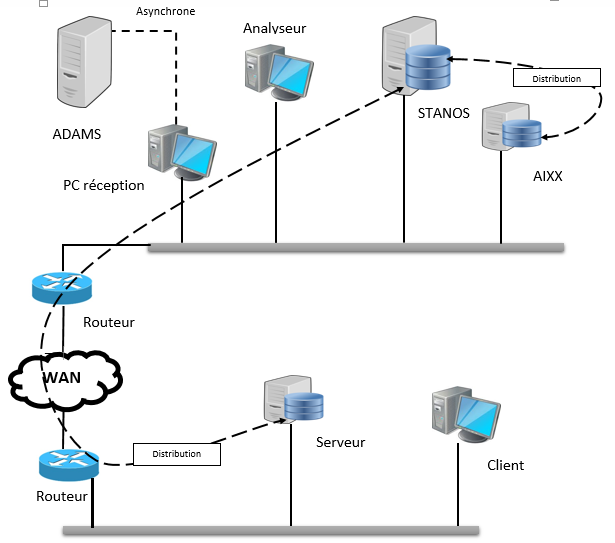
\includegraphics[width=17cm,height=6.5cm]{Conception/solution.png}
\end{center}
%légende de l'image
\caption{Schéma de la solution projetée}
\end{figure}


\subsection{Présentation de la procédure}

\subsubsection{Le site central (CNA)}
\begin{table}[!h]
\begin{center}
\begin{tabularx}{17cm}{|c|p{7.5cm}|X|}
  \hline
  \textbf{Ordre}  & \textbf{Opération à réaliser sur la base virtuelle} & \textbf{Base centrale} \\ \hline
  1 & Création du serveur virtuel AIXX & \\ \hline
  2 & Importer la base AITC ---> AIXX & \\ \hline
  3 & Vider table (NOTAM ...) et (PIB + ...) & \\ \hline
  4 & & Création de l'abonner AIXX + sa zone de couverture \\ \hline
  5 & & Exécusion de la requête SQL de création des lignes de 	distribution des NOTAMs en vigueur de l'abonné AIXX dans la table <<Distribute BNI>> \\ \hline
  6 & Lancement + Mise à jour de la base statique & \\ \hline
  7 & Réindexation & \\ \hline
  8 & Lancement de la distribution & \\ \hline
  9 & Validation & \\ \hline
  10 & Serveur AIXX opérationnel & \\ \hline
  11 & test et vérification : check-list + PIB & \\ \hline

\end{tabularx}
\end{center}
\caption{Tableau des opérations effectuées sur le site central}
\end{table}
\subsubsection{Le site distant(aéroport)}

\begin{table}[!h]
\begin{center}
\begin{tabularx}{17cm}{|c|p{7.5cm}|X|}
  \hline
  \textbf{Ordre} & \textbf{Base distante (Aéroport)} & \textbf{Base centrale} \\ \hline
  1 & Sauvegarder la base existante & \\ \hline
  2 & Supprimer la base existante (Tablespace et user) & \\ \hline
  3 & Création d'une nouvelle base vierge (Tablespace et user) & \\ \hline
  4 & Exporter AIXX crée vers la destination (selon le nom du user) & \\ \hline
  5 & Mettre à jour la table abonnée & \\ \hline
  6 & & Mise à jour la table Distribute-BNI pour redistribuer les données des N jours manquant de trafique de l'abonné \\ \hline
  7 & Lancer les modules BIA et distribution &  \\ \hline
  8 & Mise à jour des données statistique & \\ \hline
  9 & test de validation : check-list et PIB & \\ \hline
  10 & Mise en service & \\ \hline

\end{tabularx}
\end{center}
\caption{Tableau des opérations effectuées sur le site distant}
\end{table}
\newpage
\subsection{Architecture adoptée}
Nous optons pour l’architecture trois-tiers pour la mise en place de notre système. En effet, l’architecture trois-tiers est un modèle logique d’architecture applicative qui vise à séparer très nettement trois couches logicielles au sein d’une même système, à modéliser et à présenter cette application comme un empilement de trois couches. Chaque couche joue un rôle bien précis dans la conception logicielle du système :
\begin{figure}[!h]
\begin{center}
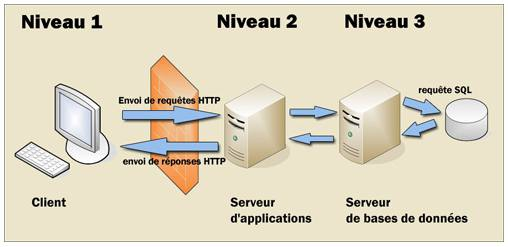
\includegraphics[width=9cm,height=4cm]{Conception/3-tiers.jpeg}
\end{center}
%légende de l'image
\caption{Architecture trois-tiers adoptée}
\end{figure}
\begin{itemize}
{\bf \item La couche présentation :} Elle correspond à la partie de l’application visible et interactive
avec les utilisateurs. On parle d’Interface Homme Machine (IHM). Elle relaie les requêtes
de l’utilisateur à destination de la couche métier, et en retour lui présente les informations
renvoyées par les traitements de cette couche.\\
Dans notre cas la couche présentation correspond à un exploitant de l'application quoiqu'il soit son type, connecté à une session après avoir être s'authentifier. 
{\bf \item La couche métier : }Elle correspond à la partie fonctionnelle de l’application, celle qui implémente
la "logique métier", et qui décrit les opérations que l’application opère sur les
données en fonction des requêtes des utilisateurs, effectuées au travers de la couche présentation.
La couche métier offre des services applicatifs à la couche présentation. Pour
fournir ces services, elle s’appuie, le cas échéant, sur les données du système, accessibles
au travers des services de la couche inférieure. En retour, elle renvoie à la couche présentation
les résultats calculés.\\
Dans notre cas la couche métier correspond au serveur de l'application  qui est chargé de traiter des
requêtes de l'agent envoyées par l’application sous forme de requêtes SQL. 
{\bf \item  La couche accès aux données :} Elle comprend la partie gérant l’accès aux gisements de
données du système. Ces données peuvent être propres au système, ou gérées par un
autre système. La couche métier n’a pas à s’adapter à ces deux cas, ils sont transparents
pour elle, et elle accède aux données de manière uniforme.\\ Dans notre cas, le serveur de base de données (Microsoft SQL Server) permet l'accès aux données stockées dans la base de données non relationnelle.
\end{itemize}
\subsection{Décomposition logique de l’application}
Nous avons utilisé côté client le framework Laravel, c’est un framework basé sur une
architecture MVC\emph ({Modèle/Vue/Contrôleur})\cite{cite3}.\\
En effet Le principe fondamental de ce pattern consiste à distinguer trois entités distinctes qui sont, le modèle, la vue et le contrôleur ayant chacun un rôle précis dans l'interface. 
Dans l'architecture MVC, les rôles des trois entités sont les suivants :

\begin{description}

 {\bf \item Rôle du modèle :}

Le modèle contient les données manipulées par le programme. Il assure la gestion de ces données et garantit leur intégrité. 
Le modèle offre des méthodes pour mettre à jour ces données (insertion suppression, changement de valeur). Il offre aussi des méthodes pour récupérer ces données. Dans le cas de données importantes, le modèle peut autoriser plusieurs vues partielles des données. 

Dans notre application, les modèles vont gérer toutes les données qui se trouvent  dans une base de données.


{\bf \item  Rôle de la vue :}

La vue fait l'interface avec l'utilisateur. Sa première tâche est d'afficher les données qu'elle a récupérées auprès du modèle. Sa seconde tâche est de recevoir toutes les actions de l'utilisateur (clic de souris, sélection d'une entrée, …) . Ces différents événements sont envoyés au contrôleur.

Dans notre application, les vues constituent les pages Web de notre site.


{\bf \item Rôle du contrôleur :}

Le contrôleur est chargé de la synchronisation du modèle et de la vue. Il reçoit tous les événements de l'utilisateur et enclenche les actions à effectuer. 
Si une action nécessite un changement de données, le contrôleur demande la modification des données au modèle et  avertit ensuite la vue que les données ont changé pour que celle-ci se mette à jour.

Dans notre application, le contrôleur va demander au modèle les données, les analyser,  prendre des décisions et renvoyer le texte à afficher à la vue. Ce contrôleur ne contient que du code en PHP et réalise des actions.

\end{description}
\section{Conception détaillée}
Dans cette partie nous allons détailler chaque composant de notre solution, précédemment décrite, d'une façon globale. 
\subsection{Conception de la base de données}
Les tables de la base de données sont les suivantes : \\

\textbf{UTILISATEUR :} c’est la table dans laquelle sont enregistrés tous les utilisateurs de l’application en précisent leurs identifications, leurs appartenances à aérodrome, et leur types.\\

\textbf{TYPE :} c’est la table des différents types des exploitants.\\

\textbf{AERODROME :} c’est la table dans laquelle existent toutes informations sur les aérodromes existant sur le FIR tunisien.\\

\textbf{HISTORIQUE :} cette table a pour but de satisfaire le besoin de sauvegarder l’historique de chaque opération effectuée ; l’agent qui l'a lancé et les administrateurs qui l’ont validé. \\

\textbf{MESSAGE :} pour garder le bon déroulement de l’opération d’apurement de base de données, on a recours à concevoir un modèle de communication entre les différents exploitants du système. Ce modèle est illustré par la table messages.\\

La relation entre ces différentes tables est illustrée par le modèle conceptuel de données suivant : \\

\begin{figure}[!h]
\begin{center}
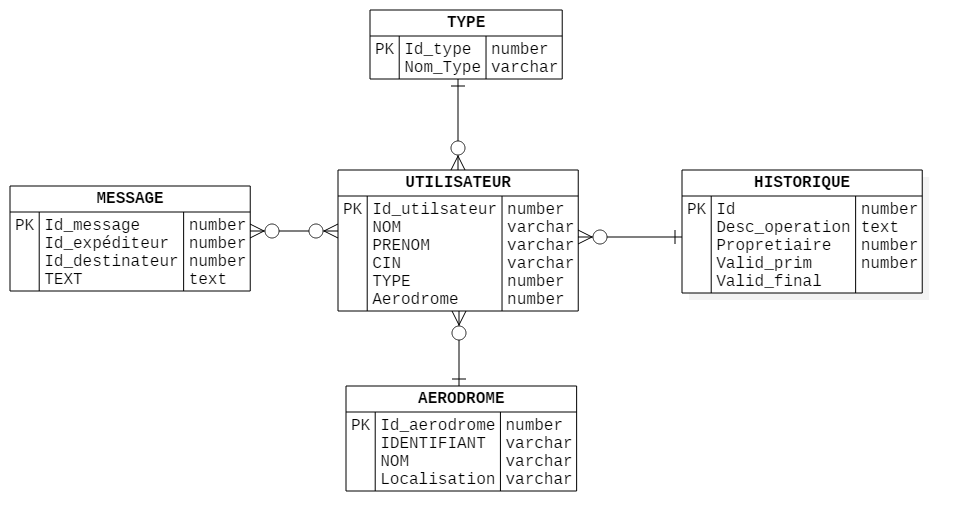
\includegraphics[width=17cm,height=12cm]{Conception/ERDDiagram1.png}
\end{center}
%légende de l'image
\caption{Modèle conceptuel de données }
\end{figure}
\newpage
\subsection{Diagramme de classe}
Notre application, conçue dans une approche orientée objet, donne naissance au diagramme de classes présenté dans la figure 4.4. \\

Une exploitant est modélisé par la classe personne, qui prend comme attribut les identifiant d’une personne. Comme il y a plusieurs types d’exploitant, trois classes hérite de la classe personne, qui sont ; AGENT, ADMINISTRATEUR et SUPER\_ADMINISTRATEUR. Ces trois classe surcharge la méthode ouvrir\_session(). Une personne peut ouvrir une seule session, pour effectuer plusieurs opérations et les inscrire dans un rapport de feedback, d’où la nécessité des classe SESSION, OPERATION et RAPPORT. Seul l’exploitant de type agent est en relation avec les messages aéronautique NOTAM, ceci s’illustre par la relation " consulter " dans le diagramme de classes.\\ 
\begin{figure}[!h]
\begin{center}
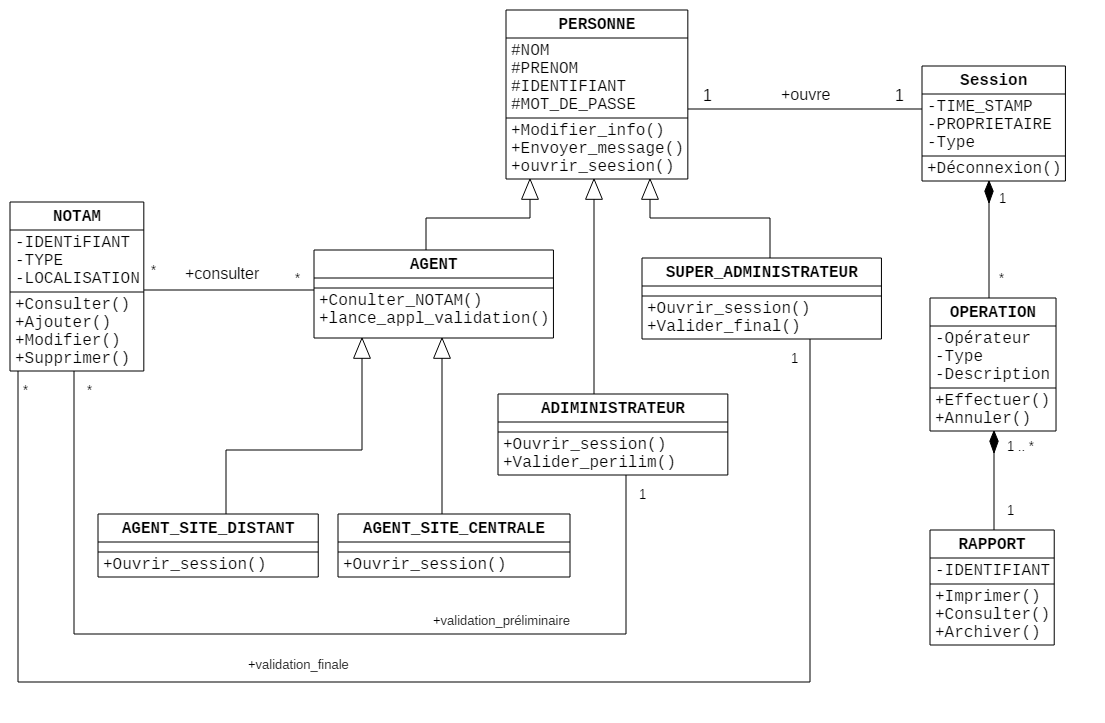
\includegraphics[width=17cm,height=13cm]{Conception/ClassDiagram1.png}
\end{center}
%légende de l'image
\caption{Diagramme de classes}

\end{figure}
\newpage
\subsection{Diagrammes de séquences}
Le déroulement général de l’opération d’apurement s’illustre dans le digramme de séquences ci-dessous, un agent lance une requête d’observation vers la base de données pour sélectionner les lignes de NOTAM à affecter. Après de vérifier, cet agent est appelé à lancer une demande de validation vers l’administrateur. S’il reçoit la validation, il peut lancer alors un bilan de l’opération vers le super-administrateur pour qu’il l’exécute et supprime les lignes expirées.\\
\begin{figure}[!h]
\begin{center}
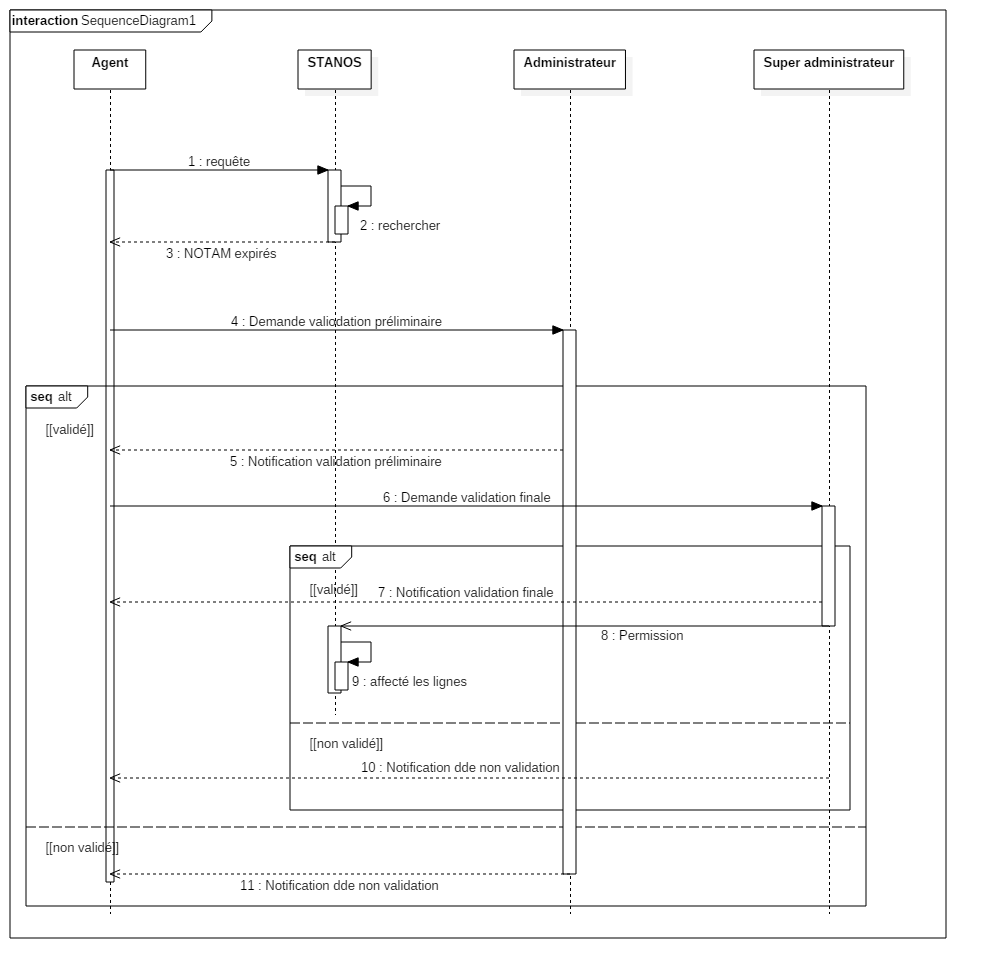
\includegraphics[width=17cm,height=18cm]{besoins/SequenceDiagram1.png}
\end{center}
%légende de l'image
\caption{Diagramme de séquences de l'opération connexion}
\end{figure}
\newpage
\section*{Conclusion}
A travers ce chapitre, nous avons présenté notre conception proposée pour l’application. Nous avons fourni, dans un premier temps, une conception globale à travers un schéma général décrivant l’organisation de notre application. Par la suite, nous avons détaillé la conception à travers quelques diagrammes UML.\\
Après avoir détaillé la conception adoptée pour la réalisation de cette application, nous décrivons dans le chapitre suivant la phase de réalisation.